%% 
%% Copyright 2007-2020 Elsevier Ltd
%% 
%% This file is part of the 'Elsarticle Bundle'.
%% ---------------------------------------------
%% 
%% It may be distributed under the conditions of the LaTeX Project Public
%% License, either version 1.2 of this license or (at your option) any
%% later version.  The latest version of this license is in
%%    http://www.latex-project.org/lppl.txt
%% and version 1.2 or later is part of all distributions of LaTeX
%% version 1999/12/01 or later.
%% 
%% The list of all files belonging to the 'Elsarticle Bundle' is
%% given in the file `manifest.txt'.
%% 
%% Template article for Elsevier's document class `elsarticle'
%% with harvard style bibliographic references

%\documentclass[preprint,12pt,authoryear]{elsarticle}

%% Use the option review to obtain double line spacing
%% \documentclass[authoryear,preprint,review,12pt]{elsarticle}

%% Use the options 1p,twocolumn; 3p; 3p,twocolumn; 5p; or 5p,twocolumn
%% for a journal layout:
%% \documentclass[final,1p,times,authoryear]{elsarticle}
%% \documentclass[final,1p,times,twocolumn,authoryear]{elsarticle}
%% \documentclass[final,3p,times,authoryear]{elsarticle}
%% \documentclass[final,3p,times,twocolumn,authoryear]{elsarticle}
%% \documentclass[final,5p,times,authoryear]{elsarticle}
 \documentclass[final,5p,times,twocolumn, nopreprintline]{elsarticle}

%% For including figures, graphicx.sty has been loaded in
%% elsarticle.cls. If you prefer to use the old commands
%% please give \usepackage{epsfig}

%% The amssymb package provides various useful mathematical symbols
\usepackage{amssymb}
\usepackage{lipsum}
\usepackage{amsmath}
%\usepackage[pdftex,active,tightpage]{preview}
%\setlength\PreviewBorder{2mm}

\usepackage{pgfplots}
\usepackage{tikz}
\usetikzlibrary{calc}
\usetikzlibrary{patterns}
\pgfplotsset{compat=1.10}
\usepgfplotslibrary{fillbetween}
%% The amsthm package provides extended theorem environments
%% \usepackage{amsthm}

%% The lineno packages adds line numbers. Start line numbering with
%% \begin{linenumbers}, end it with \end{linenumbers}. Or switch it on
%% for the whole article with \linenumbers.
%% \usepackage{lineno}

%% You might want to define your own abbreviated commands for common used terms, e.g.:
\newcommand{\kms}{km\,s$^{-1}$}
\newcommand{\msun}{$M_\odot}
\newcommand{\toplrarr}[1]{\overset{\text{\scriptsize$\leftrightarrow$}}{#1}}
\numberwithin{equation}{section}
%\journal{Astronomy $\&$ Computing}

\begin{document}

\begin{frontmatter}

%% Title, authors and addresses

%% use the tnoteref command within \title for footnotes;
%% use the tnotetext command for theassociated footnote;
%% use the fnref command within \author or \affiliation for footnotes;
%% use the fntext command for theassociated footnote;
%% use the corref command within \author for corresponding author footnotes;
%% use the cortext command for theassociated footnote;
%% use the ead command for the email address,
%% and the form \ead[url] for the home page:
%% \title{Title\tnoteref{label1}}
%% \tnotetext[label1]{}
%% \author{Name\corref{cor1}\fnref{label2}}
%% \ead{email address}
%% \ead[url]{home page}
%% \fntext[label2]{}
%% \cortext[cor1]{}
%% \affiliation{organization={},
%%            addressline={}, 
%%            city={},
%%            postcode={}, 
%%            state={},
%%            country={}}
%% \fntext[label3]{}

\title{A review on Dark Matter production mechanisms}

%% use optional labels to link authors explicitly to addresses:
%% \author[label1,label2]{}
%% \affiliation[label1]{organization={},
%%             addressline={},
%%             city={},
%%             postcode={},
%%             state={},
%%             country={}}
%%
%% \affiliation[label2]{organization={},
%%             addressline={},
%%             city={},
%%             postcode={},
%%             state={},
%%             country={}}

\author[first]{Santiago Julio Dávila}
\affiliation[first]{organization={Institute of Physics, University of Antioquia},%Department and Organization
            city={Medellín},
            state={Antioquia},
            country={Colombia}}

\begin{abstract}
%% Text of abstract

\end{abstract}

%%Graphical abstract
%\begin{graphicalabstract}
%\includegraphics{grabs}
%\end{graphicalabstract}

%%Research highlights
%\begin{highlights}
%\item Research highlight 1
%\item Research highlight 2
%\end{highlights}

\begin{keyword}
%% keywords here, in the form: keyword \sep keyword, up to a maximum of 6 keywords

%% PACS codes here, in the form: \PACS code \sep code

%% MSC codes here, in the form: \MSC code \sep code
%% or \MSC[2008] code \sep code (2000 is the default)

\end{keyword}


\end{frontmatter}

%\tableofcontents

%% \linenumbers

%% main text

\section{Introduction}

[Introduction goes here]

\section{Boltzmann equation}

To study the evolution of different energy components in the Universe it is necessary to consider departures from thermal equilibrium. A rough criterion to establish the moment in which a species is no longer in thermal equilibrium, or \emph{decouples}, is given in terms of the interaction rate of the particles, $\Gamma$ and the expansion rate of the universe, $H$:

\begin{align}
\Gamma&\gtrsim H \text{ (coupled)}\nonumber\\
\Gamma&\lesssim H \text{ (decoupled)}, \label{eq:decoupling}
\end{align}

that is, the species decouples from the thermal bath when the Hubble expansion rate is higher than the interaction rate of the particles. In order to track the evolution of the number density of the particles of interest, we need an equation describing the evolution of phase space distribution, $f(x^\mu,p^\mu)$, of the particle. Said equation is known as the Boltzmann equation, which, in general can be written as

\begin{equation}
\hat{\mathcal{L}}\{f\}=\mathcal{C}\{f\},\label{eq:Boltz_gen}
\end{equation}

where $\hat{\mathcal{L}}$ is the Liouville operator and $\mathcal{C}\{f\}$ is the collision term \cite{kolb1991early}.

\subsection{Liouville operator}

The Liouville operator can be defined as a total derivative with respect to a parameter of a function whose variables can depend on that parameter implicitly. In classical mechanics, the parameter is usually the time, and the Liouville operator is generally applied over a function $f(\vec{x},\vec{v},t)$, hence the Liouville operator takes the form

\begin{equation}
\hat{\mathcal{L}}_{c}=\dfrac{\partial}{\partial t}+\dot{\vec{x}}\cdot\nabla+\dot{\vec{v}}\cdot\nabla_{\vec{v}}. \label{eq:clas_liouville}
\end{equation}

Extending this definition to general relativity is straightforward, choosing a parameter $\theta$ such that $\frac{\mathrm{d}x^\mu}{\mathrm{d}\theta}\equiv\dot{x}^\mu=p^\mu$ and considering functions of the type $f(x^\mu,p^\mu)$ that do not depend explicitly on said parameter, the Liouville operator is given by

\begin{equation}
\hat{\mathcal{L}}=p^\mu\dfrac{\partial}{\partial x^\mu}-\Gamma^\mu_{\alpha\beta}p^\alpha p^\beta \dfrac{\partial}{\partial p^\mu}, \label{eq:rel_liouville}
\end{equation}

where we have used the geodesic equation $\dot{p}^\mu+\Gamma^\mu_{\alpha\beta}p^\alpha p^\beta=0$ \cite{bichteler1967cauchy}. The distribution functions of interest are homogeneous and isotropic in space, as determined by the Friedmann-Lemaître-Robertson-Walker (FLRW) metric: $f(x^\mu,p^\mu)=f(x^0,p^0)=f(t,E)$. With this metric, it is easy to verify that the Liouville operator is

\begin{equation}
\hat{\mathcal{L}}\{f\}=E\dfrac{\partial f}{\partial t}-\dfrac{\dot{a}}{a}p^2\dfrac{\partial f}{\partial E}. \label{eq:flrw_liouville}
\end{equation}

Integrating this expression over $\mathrm{d}\tilde{p}=\frac{g}{(2\pi)^3}\frac{\mathrm{d}^3\vec{p}}{E}$ and using the definition of number density

\begin{equation}
n(t)=\dfrac{g}{(2\pi)^3}\int\mathrm{d}^3\vec{p}f(E,t), \label{eq:num_dens}
\end{equation}

where $E$ is subject to the constraint $E^2=m^2+p^2$, the Boltzmann equation reads

\begin{equation}
\dfrac{\mathrm{d}n}{\mathrm{d}t}+3Hn=\dfrac{g}{(2\pi)^3}\int\mathrm{d}^3\vec{p}\dfrac{\mathcal{C}\{f\}}{E}. \label{eq:Boltz_lhs}
\end{equation}

Defining $Y=n/s$ and $x=m/T$, where 

\begin{equation}
s=\dfrac{2\pi²}{45}g_{\star s}(T)T^3 \label{eq:ent_dens}
\end{equation}

is the entropy density \cite{baumann2022cosmology} satisfying entropy conservation $sa^3=constant$, hence, ignoring the temperature dependence of $g_{\star s}$, $\dot{s}=-3Hs$. Differentiating $Y$ with respect to time

\begin{equation}
\dot{Y}=\dfrac{\dot{n}}{s}-\dfrac{n\dot{s}}{s^2}=\dfrac{\dot{n}+3Hn}{s}. \label{eq:Ydot}
\end{equation}

From entropy conservation, using the functional form of $s$ and neglecting the temperature dependence of $g_\star$, we can also deduce $aT=constant$, and so, $\dot{T}=-HT$. Using the chain rule, one could write the time derivative in terms of the variable $x$: $\frac{\mathrm{d}}{\mathrm{d}t}=\frac{\mathrm{d}T}{\mathrm{d}t}\frac{\mathrm{d}x}{\mathrm{d}T}\frac{\mathrm{d}}{\mathrm{d}x}=Hx\frac{\mathrm{d}}{\mathrm{d}x}$, so the Boltzmann equation can be written as \cite{mambrini2021particles}

\begin{equation}
\dfrac{\mathrm{d}Y}{\mathrm{d}x}=\dfrac{1}{Hxs}\dfrac{g}{(2\pi)^3}\int\mathrm{d}^3\vec{p}\dfrac{\mathcal{C}\{f\}}{E}. \label{eq:Boltz_Y}
\end{equation}

\subsection{Collision term}

Considering a reaction $\underbrace{\psi+a+b+...}_{in}\rightleftharpoons \underbrace{i+j+...}_{out}$, where $\psi$ is the species of interest. The collision term for a process like this is given by

\begin{align}
\int\mathcal{C}\{f\}\mathrm{d}\tilde{p}_\psi=&-\dfrac{1}{Hxs}\int\left(\prod_{in}\mathrm{d}\tilde{p}_k\right)\left(\prod_{out}\mathrm{d}\tilde{p}_k\right)(2\pi)^4\delta^4(p_{in}-p_{out})\times\nonumber\\
&\times\left[|M|^2_\rightarrow\left(\prod_{in}f_k\right)\left(\prod_{out}(1\pm f_k)\right)\right.-\nonumber\\
&-\left.|M|^2_\leftarrow\left(\prod_{out}f_k\right)\left(\prod_{in}(1\pm f_k)\right)\right], \label{eq:collision_gen}
\end{align}

which can be simplified by considering $CP$ invariance, which implies the invariant transition amplitude for the forward reaction is equal to that of the reverse reaction: $|M|^2_\rightarrow=|M|^2_\leftarrow=|M|^2$, and by ignoring the blocking and stimulated emission factors $1\pm f_k\simeq 1$, leading to the Boltzmann equation \cite{kolb1991early}

\begin{align}
\dfrac{\mathrm{d}Y}{\mathrm{d}x}=&-\dfrac{1}{Hxs}\int\left(\prod_{in}\mathrm{d}\tilde{p}_k\right)\left(\prod_{out}\mathrm{d}\tilde{p}_k\right)(2\pi)^4\delta^4(p_{in}-p_{out})\times\nonumber\\&\times|M|^2\left[\left(\prod_{in}f_k\right)-\left(\prod_{out}f_k\right)\right]. \label{eq:collision_sim}
\end{align}

We shall focus our attention in some particle-like dark matter (DM) candidates, and the solutions to Boltzmann equation in said context. The first DM model to be analyzed are \emph{Weakly Interacting Massive Particles}, or WIMPs, which decouple from the thermal bath mainly via $2\rightarrow2$ annihilations into standard model (SM) particles, and satisfy the relic density constraint from observational data $\Omega_0 h^2\simeq0.12$; there are other alternate mechanisms from which WIMPs freeze-out, such as semi-annihilation, which will be discussed here \cite{bhattacharya2020simpler}. Another mechanism that can produce the observed relic density is the freeze-in mechanism, in which the coupling between the dark sector and the visible sector is small enough to prevent the dark sector to be in thermal equilibrium with the dark sector, and the relic abundance freezes to a constant value after the densities of the visible particles producing the dark particles becomes Boltzmann-suppressed; dark particles produced by this mechanism are called \emph{Frozen-In} or \emph{Feebly Interacting Massive Particles}, FIMPs for short \cite{bernal2017dawn}. If we assume very small DM-SM interactions, self-interactions within the dark sector become significant, in particular, number-changing processes, such as $3\to2$, which we will study here, and $4\to2$; this alternative channel is related to \emph{Strongly Interacting Massive Particles}, or SIMPs \cite{bhattacharya2020simpler}.

\section{Boltzmann equation for WIMPs}

\subsection{Annihilation}


\begin{figure}[h]
\begin{center}
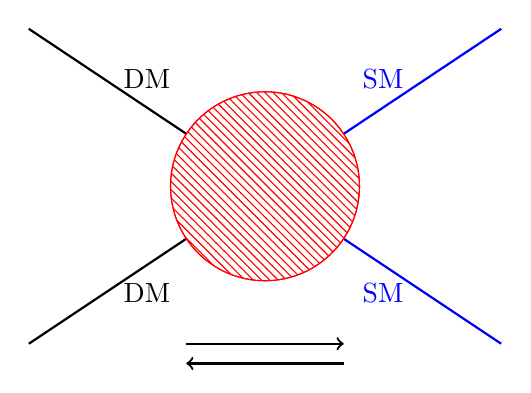
\begin{tikzpicture}
    \newcommand{\R}{1.2}
    \path (240:\R) coordinate (A);
    \path ( 60:\R) coordinate (B);
    \path ( 0:\R) coordinate (C);
    %\draw[help lines,line width=0.1pt,blue] (-3, -2) grid (3, 2);
	\draw[thick,black] (-3,-2)--(0,0) node[midway,below=3pt]{DM};
	\draw[thick,black] (-3,2)--(0,0) node[midway,above=3pt]{DM};
	\draw[thick,blue] (3,2)--(0,0) node[midway,above=3pt]{SM};
	\draw[thick,blue] (3,-2)--(0,0) node[midway,below=3pt]{SM};
	\draw[red,fill=white] (0,0) circle (\R);
	\draw[red,fill=white,pattern=north west lines, pattern color=red] (0,0) circle (\R);
	\draw[thick,black,->] (-1,-2)--(1,-2);
	\draw[thick,black,<-] (-1,-2.25)--(1,-2.25);
\end{tikzpicture}
\end{center}
\caption{$2\to2$ WIMP annihilation.}
\end{figure}\label{fig:wimp_an}

We will first consider the WIMP annihilation into SM particles $DM+DM\rightleftharpoons SM+SM$ happenning during the radiation domination epoch, described by the Friedmann equation

\begin{equation}
H(T)=\sqrt{\dfrac{\rho_R(T)}{3M_P^2}}, \label{eq:hubble_rate}
\end{equation}

where $M_P\approx 2.4\times10^{18}\text{ GeV}$ is the reduced Planck mass \cite{mambrini2021particles}, $g_\star=106.75$, and the SM radiation energy density is given by

\begin{equation}
\rho_R(T)=\dfrac{\pi^2}{30}g_\star T^4. \label{eq:rad_dens}
\end{equation}

The collision term for this process is given by \cite{baumann2022cosmology}

\begin{align}
\int\mathcal{C}\{f\}\mathrm{d}\tilde{p}=&-\int\mathrm{d}\tilde{p}_1\mathrm{d}\tilde{p}_2\mathrm{d}\tilde{p}_3\mathrm{d}\tilde{p}_4(2\pi)^4\delta^4(p_1+p_2-p_3-p_4)\times\nonumber\\&\times|M|^2(f_1f_2-f_3^{eq}f_4^{eq}), \label{eq:col_22}
\end{align}

where 1 and 2 represent the DM particles on the left side of the reaction and 3 and 4 represent the SM particles on the right side of the reaction, which are in thermal equilibrium, thus, the superindex ``q'' on $f_3^{eq}f_4^{eq}$. The Dirac delta accounts for the conservation of the 4-momentum in the process, particularly, the conservation of energy. We assume that the equilibrium distributions are Maxwell-Boltzmann distributions without chemical potential \cite{kolb1991early}: $f_i^{eq}\sim \exp(-E_i/T)$ and the non-equilibrium distributions are approximately proportional to the equilibrium distributions $f_i\approx\left(\frac{n_i}{n_i^{eq}}f_i^{eq}\right)$ \citep{pierre2019dark}. The SM particles distributions is then

\begin{equation}
f_3^{eq}f_4^{eq}=\exp\left(-\dfrac{E_3+E_4}{T}\right)=\exp\left(-\dfrac{E_1+E_2}{T}\right)=f_1^{eq}f_2^{eq}. \label{eq:eq_dist_wimp}
\end{equation}

Replacing in the equation \ref{eq:col_22}, we get the expression

\begin{align}
\int\mathcal{C}\{f\}\mathrm{d}\tilde{p}&=-(n_1n_2-n_1^{eq}n_2^{eq})\dfrac{1}{n_1^{eq}n_2^{eq}}\int\mathrm{d}\tilde{p}_1\mathrm{d}\tilde{p}_2\mathrm{d}\tilde{p}_4\mathrm{d}\tilde{p}_3(2\pi)^4\times\nonumber\\&\times\delta^4(p_1+p_2-p_3-p_4)|M|^2f_1^{eq}f_2^{eq}\nonumber\\&=-\langle\sigma v\rangle(n^2-n_{eq}^2), \label{eq:col_22_n}
\end{align}

where the thermally-averaged cross section, $\langle\sigma v\rangle$, is defined as the integral in equation \ref{eq:col_22_n} and we have used the fact that there is no asymmetry between the DM species involved in the reaction, hence $n_1=n_2=n$. $n_{eq}$ is easily found considering that the equilibrium distributions are Maxwell-Boltzmann distributions \cite{baumann2022cosmology}:

\begin{equation}
n_{eq} = \dfrac{g}{2\pi^2}m^2TK_2\left(\dfrac{m}{T}\right). \label{eq:neq}
\end{equation}

 Using the definition of $Y$, the Boltzmann equation becomes 

\begin{equation}
\dfrac{\mathrm{d}Y}{\mathrm{d}x}=-\dfrac{\langle\sigma v\rangle s}{Hx}(Y^2-Y_{eq}^2). \label{eq:Boltz_wimp}
\end{equation}

and the relic abundance $\Omega_0=mY_0s_0/3H_0^2M_P^2$ is given by:

\begin{equation}
\Omega_{0}h^2=\dfrac{Y_0ms_0}{3M_P^2(2.13\times 10^{-42}\text{ GeV})^2}, \label{eq:omegah2}
\end{equation}

where the subscript 0 represents the current value of the quantity in question \cite{mambrini2021particles}. An approximate analytic solution for the relic abundance can be obtained from \ref{eq:Boltz_wimp} by making some considerations on $Y$ and $Y_{eq}$. We shall assume that the freeze-out occurs when the DM particles are non-relativistic ($x_f\gtrsim3$), producing cold relics \cite{kolb1991early}. For temperatures higher than a few MeV, the approximation $g_{\star s}=g_\star$ works well, and so, the factor $\frac{\langle\sigma v\rangle s}{Hx}$ can be rewritten in terms of $x$ and constants

\begin{equation}
\dfrac{\langle\sigma v\rangle s}{Hx}=\dfrac{2}{15}\langle\sigma v\rangle\sqrt{10g_\star}M_Pmx^{-2}=\lambda x^{-2}, \label{eq:factor}
\end{equation}

and, for $x\gg3$

\begin{equation}
Y_{eq}\approx\dfrac{45}{2\pi^4}\dfrac{g}{g_\star}\sqrt{\dfrac{\pi}{8}}x^{3/2}e^{-x}. \label{eq:Yeq_lat}
\end{equation}

Under this approximation, $Y_{eq}'\approx-Y_{eq}$
\bibliographystyle{abbrv} 
\bibliography{reviewdm.bib}

%% else use the following coding to input the bibitems directly in the
%% TeX file.

%%\begin{thebibliography}{00}

%% \bibitem[Author(year)]{label}
%% For example:

%% \bibitem[Aladro et al.(2015)]{Aladro15} Aladro, R., Martín, S., Riquelme, D., et al. 2015, \aas, 579, A101


%%\end{thebibliography}

\end{document}

\endinput
%%
%% End of file `elsarticle-template-harv.tex'.
